Justificación de las técnicas y tecnologías empleadas en el trabajo, especificando las razones por las que se han descartado otras igualmente aplicables.

\section{Metodología}

En este apartado se especificarán las fases del trabajo, así como la metodología o metodologías empleadas para desarrollar cada una de las fases. 

\newpage

\section{Tecnologías empleadas}

Las tecnologías utilizadas para el desarrollo de la aplicación se pueden clasificar según su uso. Debido a que el formato propuesto para el desarrollo es similar al de un videojuego, donde la interacción es esencial para su uso correcto y óptimo, se ha seleccionado software adecuado para el producto realizado. A continuación, se explicará detalladamente el uso de las diferentes tecnologías y las razones detrás de la elección de cada una específicamente.

\subsection{Unity}

Un motor de videojuegos, del inglés game engine, es un entorno que proporciona un conjunto de herramientas reutilizables que facilitan la creación de videojuegos a los desarrolladores. Estos se pueden dividir en el motor gráfico, responsable del aspecto visual, y el motor físico, encargado de dotar al motor de leyes físicas como la gravedad, la masa o las fuerzas. Cada motor de videojuegos tiene sus propios usos y limitaciones. Por lo tanto, la elección del motor a utilizar es de gran importancia antes de iniciar el desarrollo. Existen motores más especializados en el desarrollo 3D como \textit{Unreal Engine} (\cite{UE:1998}), mientras que otros están centrados en gráficos 2D, como \textit{Game Maker Studio} (\cite{GMS:1999}) y \textit{RPG Maker} (\cite{RPGM:1992}). \textit{Unity} (\cite{UNITY:2005}) y \textit{Godot Engine} (\cite{GODOT:2001}) son híbridos que permiten el desarrollo en ambas dimensiones.

Unity, junto con Unreal Engine y recientemente Godot Engine, es uno de los motores de videojuegos más populares en la industria. Aunque Unreal Engine es valorado como posiblemente el mejor motor de videojuegos de la actualidad, su uso está limitado a circunstancias muy específicas: videojuegos 3D para consolas de última generación. Sin embargo, Unity, aunque no ofrece la potencia gráfica de Unreal Engine, es mucho más versátil y se puede utilizar en una amplia variedad de circunstancias. Esto permite que el rango de plataformas para las que se puede desarrollar con este motor aumente, convirtiéndolo en una opción más segura para enfocarse en el desarrollo multiplataforma.

\begin{figure}[h!]
	\centering
	\subfigure[Unity.]{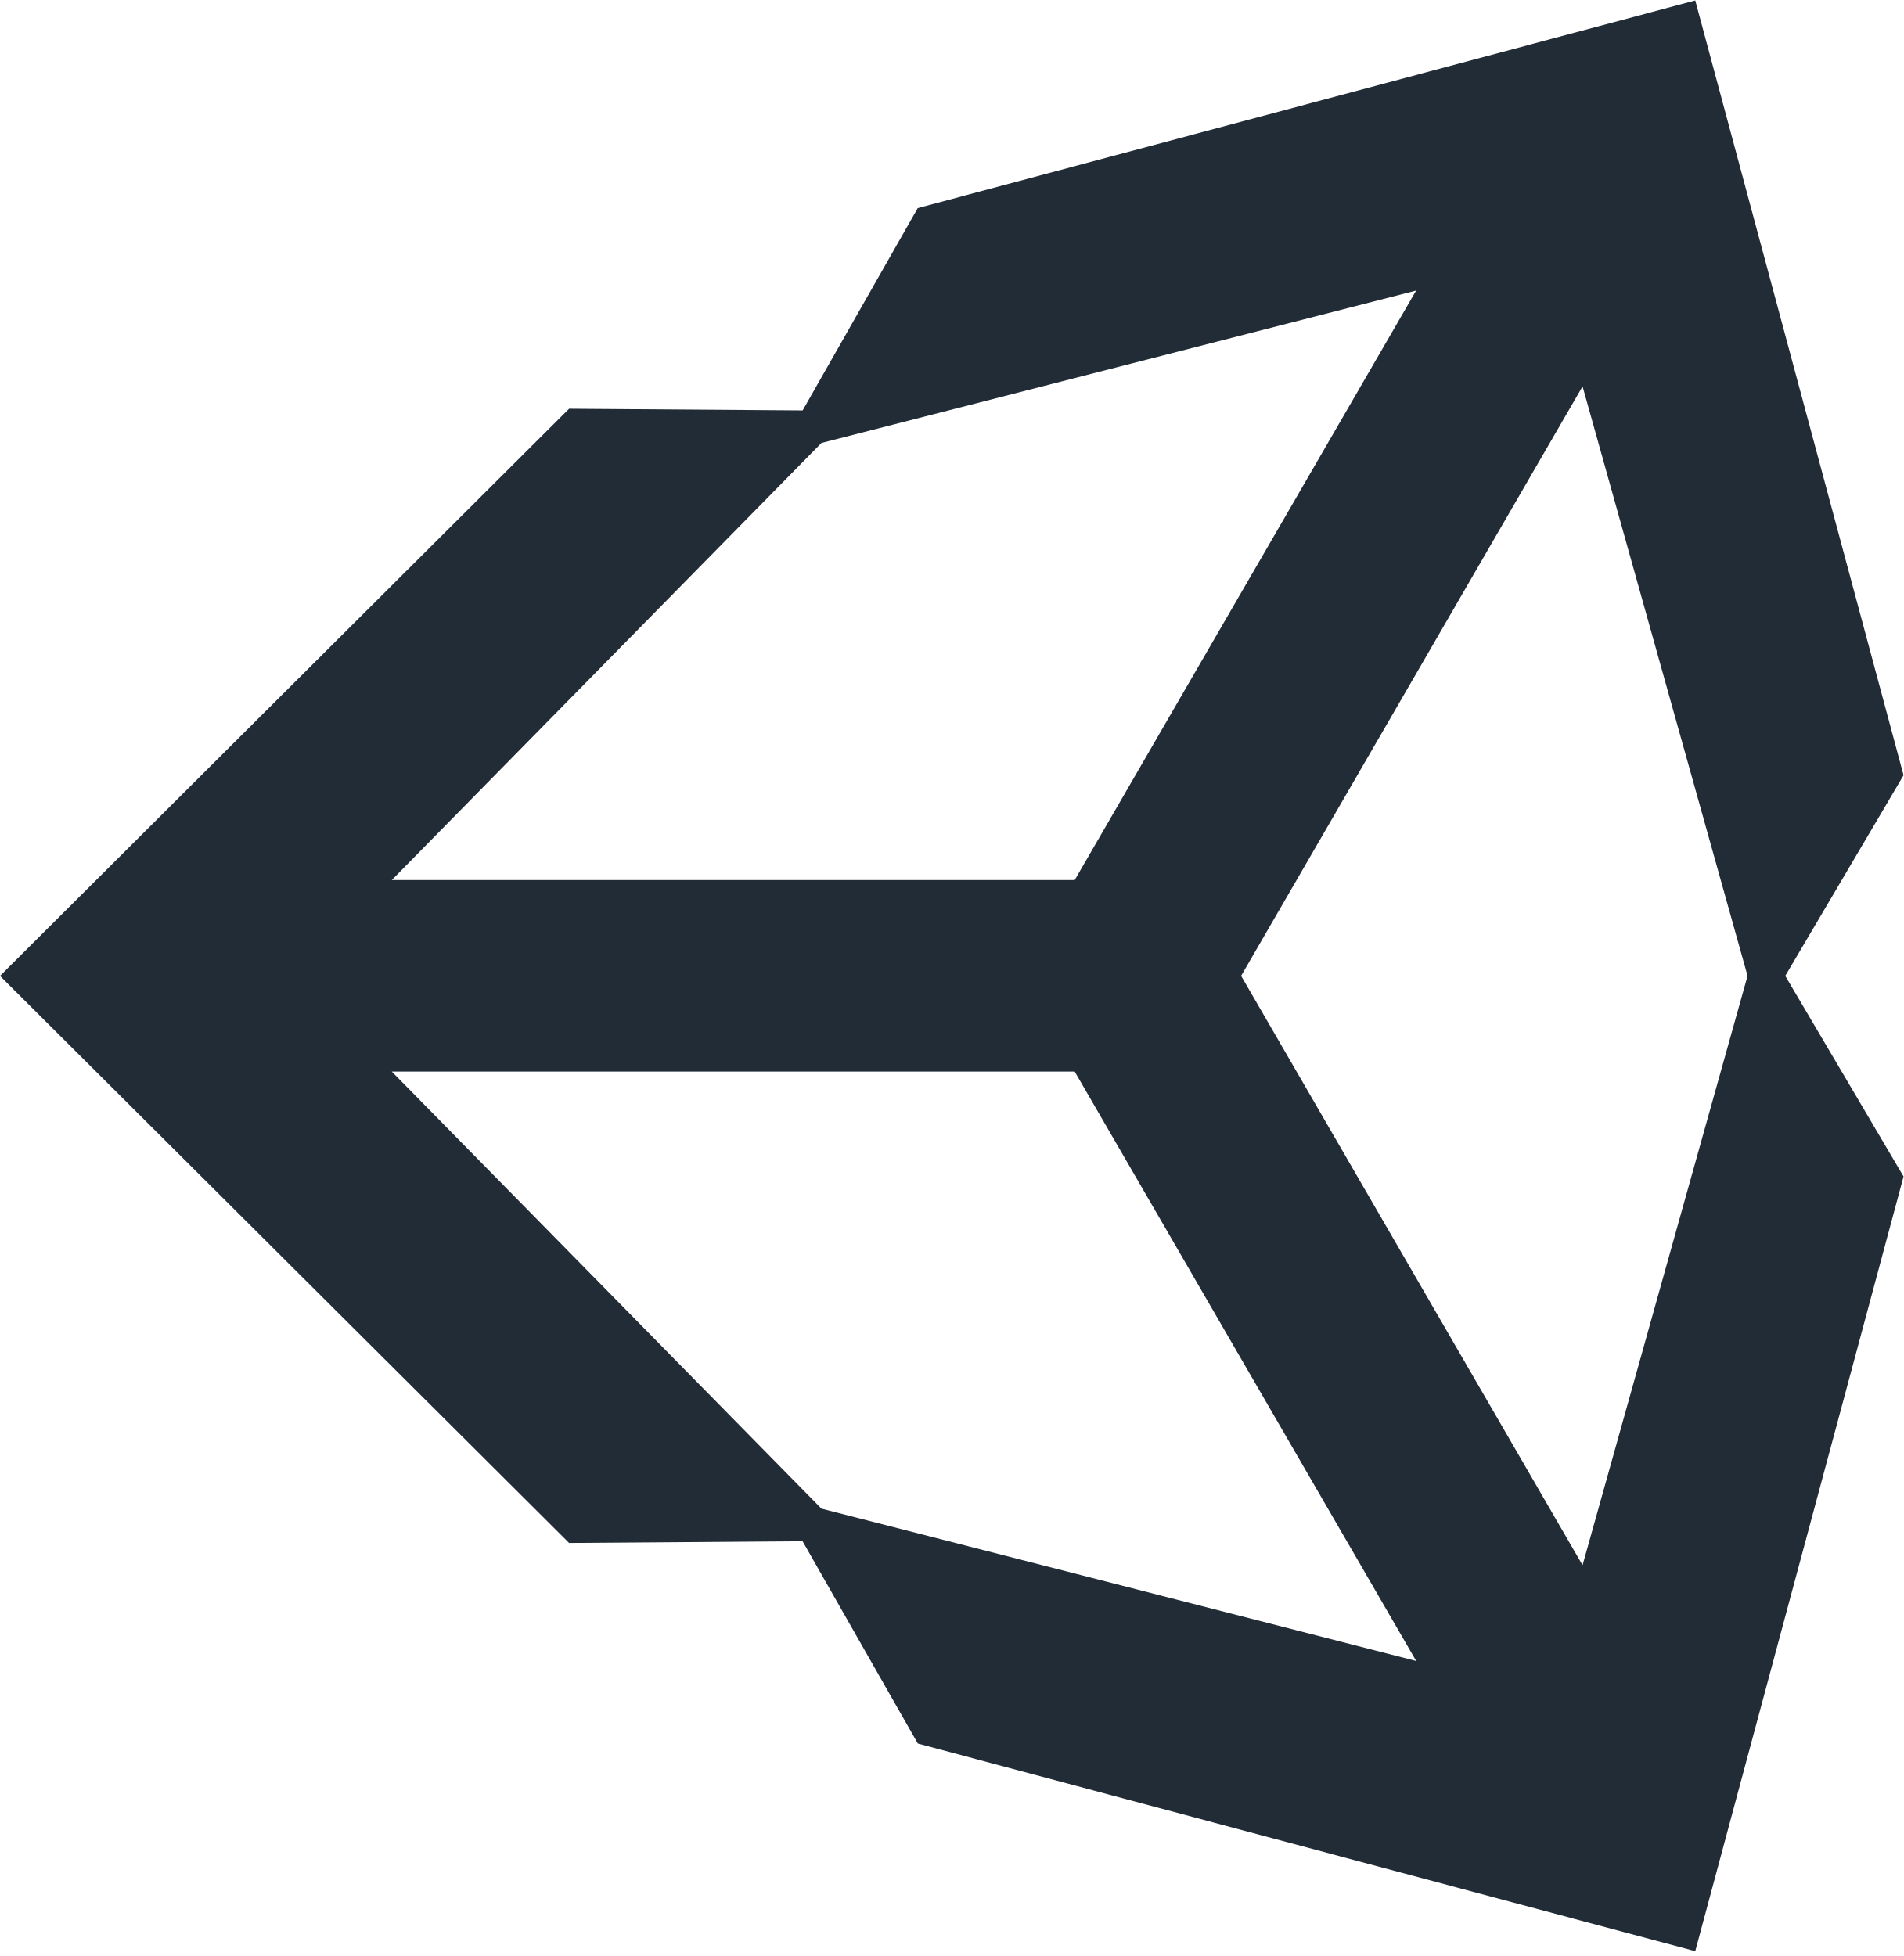
\includegraphics[width=0.2\textwidth]{./Figuras/Aspectos/UnityLogo}\label{fig:UnityLogo}}
	\hfil
	\subfigure[Unreal Engine.]{
\includegraphics[width=0.2\textwidth]{./Figuras/Aspectos/UnrealLogo.png}\label{fig:UnrealLogo}}
	\hfil
	\subfigure[Godot Engine.]{
\includegraphics[width=0.2\textwidth]{./Figuras/Aspectos/GodotLogo.png}\label{fig:GodotLogo}}
	\caption{Logotipos de los motores de videojuegos mencionados en el párrafo anterior.}
	\label{fig:GameEngineLogos}
\end{figure}

Hemos seleccionado Unity para nuestro caso específico por diversas razones, dado que la aplicación se desarrolla completamente en 2D y nuestra plataforma objetivo son los dispositivos móviles, en particular las tabletas. Unity domina el 50\% del desarrollo de videojuegos para móviles, consolas y PC, con un 71\% de los 1000 mejores juegos móviles creados en Unity (\cite{PLARIUM:2024}).

El motor gráfico 2D de Unity ofrece diversas herramientas útiles para el desarrollo, como el Sprite Editor. Además, Unity tiene una sólida integración de físicas 2D que permite simular colisiones, gravedad y otros elementos físicos. Su interfaz es intuitiva y fácil de usar, como se muestra en la \autoref{fig:UnityUI}, facilitando la creación rápida de videojuegos.

\begin{figure}[h!]
	\centering
	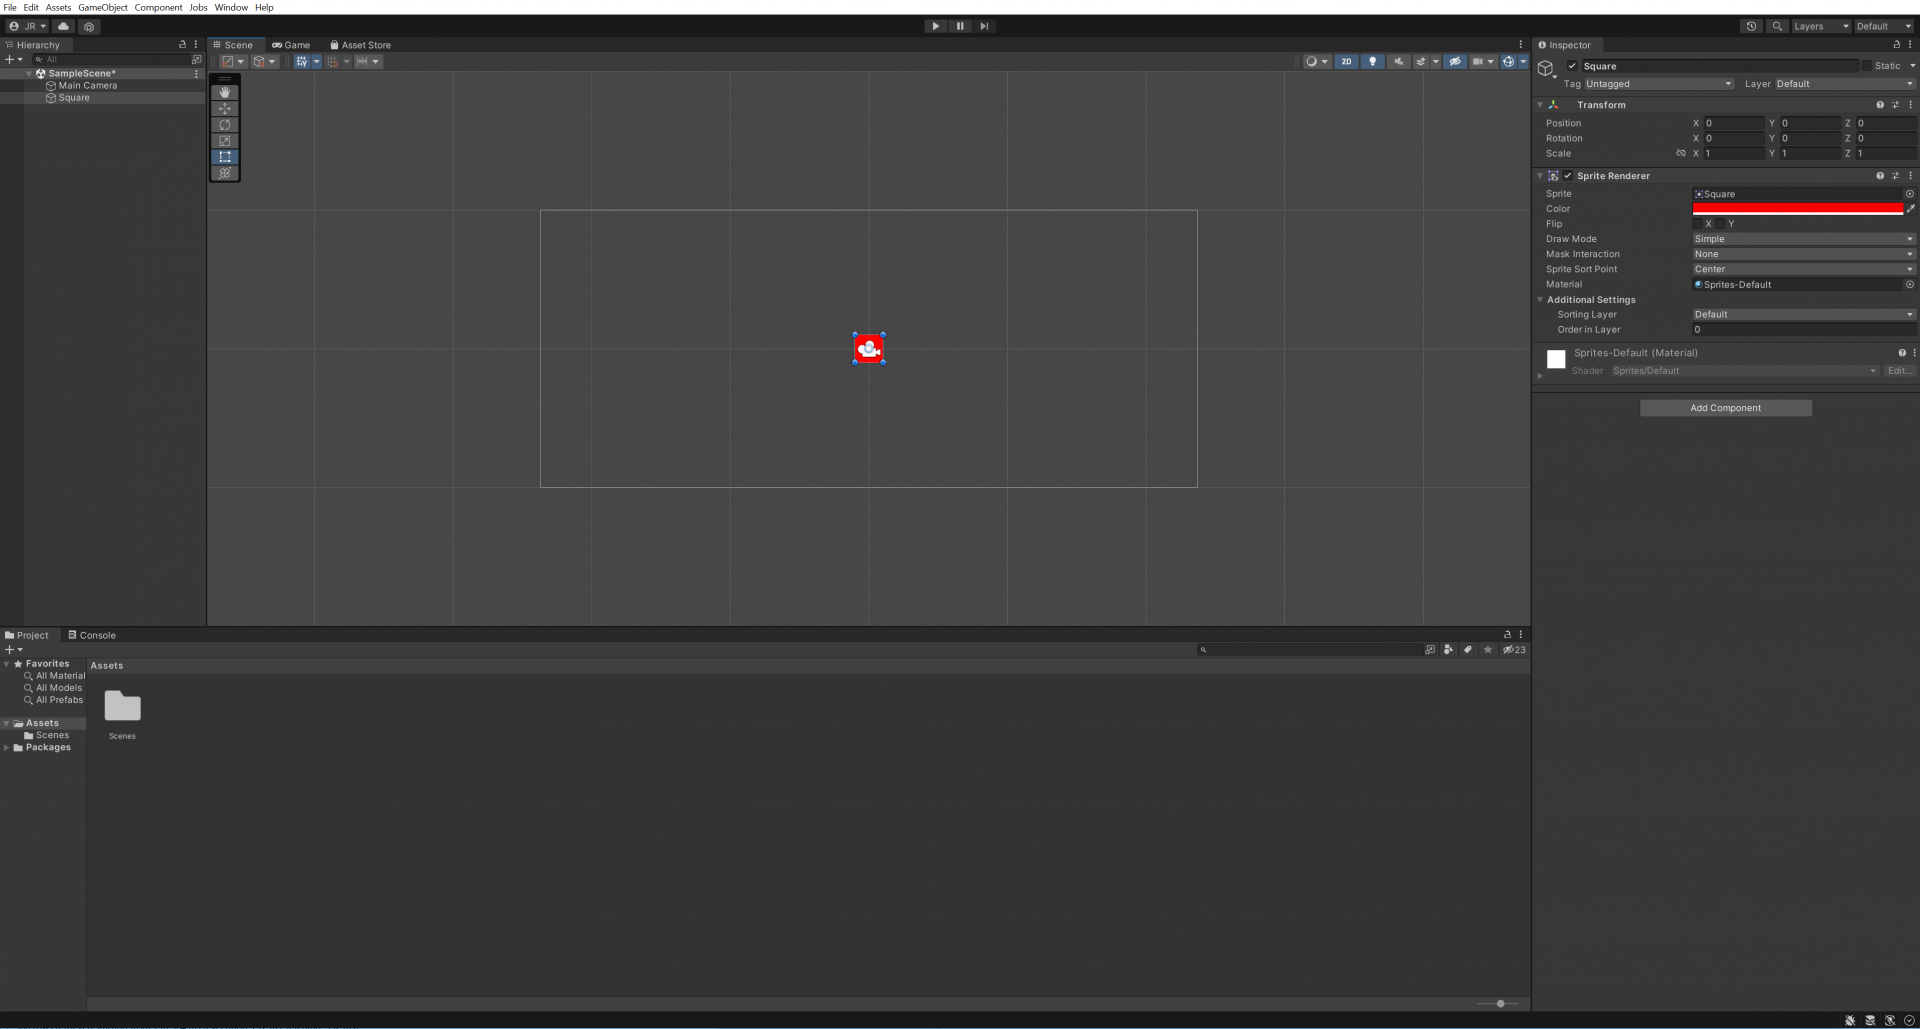
\includegraphics[width=0.8\linewidth]{./Figuras/Aspectos/UnityUI.png}
	\caption{Interfaz de usuario de la plantilla 2D de Unity.}
	\label{fig:UnityUI}
\end{figure}

La capacidad de arrastrar y soltar objetos en el editor de Unity simplifica significativamente el proceso de diseño, permitiendo a los desarrolladores centrarse en la creatividad y la jugabilidad en lugar de en aspectos técnicos complejos. Además, Unity cuenta con una comunidad amplia y activa que ofrece acceso a foros, tutoriales, cursos en línea y documentación extensa. Esta comunidad es un recurso invaluable para obtener soporte y encontrar soluciones a problemas comunes, aprender técnicas nuevas y compartir experiencias.

La Asset Store de Unity ofrece una gama variada de recursos como sprites, animaciones, scripts y plugins, que pueden agilizar el desarrollo. Estos recursos preconstruidos permiten a los desarrolladores integrar rápidamente elementos visuales y funcionales complejos sin la necesidad de crearlos desde cero, ahorrando tiempo y esfuerzo.

Todos estos factores, sumados a que Unity es el motor en el que más experiencia tenemos, fueron decisivos para seleccionarlo como el motor de desarrollo para ARTEMIS. La versión seleccionada es la 2021.3.31f, que fue la última versión de soporte a largo plazo (LTS) disponible en el momento en que se inició el proyecto.

\subsection{Visual Studio 2022}

Visual Studio es un entorno de desarrollo integrado (IDE) y editor de código, creado por Microsoft en 1997. Este editor es compatible con numerosos lenguajes de programación, como C++, Visual Basic .NET, Fortran, J\# y, más relevante para nuestro desarrollo, C\#. Su versión 2022 es la última versión disponible actualmente, y ha incorporado mejoras de rendimiento y nuevas funciones de accesibilidad para el usuario. Visual Studio, junto con Visual Studio Code y JetBrains Rider, forma el conjunto de editores de código con la mejor integración con Unity.

\subsection{FMOD}

FMOD Studio es un middleware\footnote{Un middleware, en términos de informática, es un software que facilita la comunicación entre las distintas aplicaciones y el sistema operativo. Además, proporciona funcionalidades inteligentes que permiten una innovación más rápida y un desarrollo eficiente. En el desarrollo de videojuegos, el middleware es un software que facilita la implementación de funcionalidades específicas dentro del motor.} de audio para videojuegos. Fue desarrollado y lanzado por Fireflight Technologies en 1995. Este motor de música y efectos de sonido se asemeja a un DAW tradicional, como se puede observar en la \autoref{fig:FMODUI}. FMOD Studio pertenece a la misma familia que el middleware Audiokinetic Wwise. Ambos proveen herramientas para la sonorización de videojuegos que facilitan la implementación de audio. Sin embargo, se ha decidido utilizar FMOD Studio debido a la mayor familiaridad con este software.

\begin{figure}[h!]
	\centering
	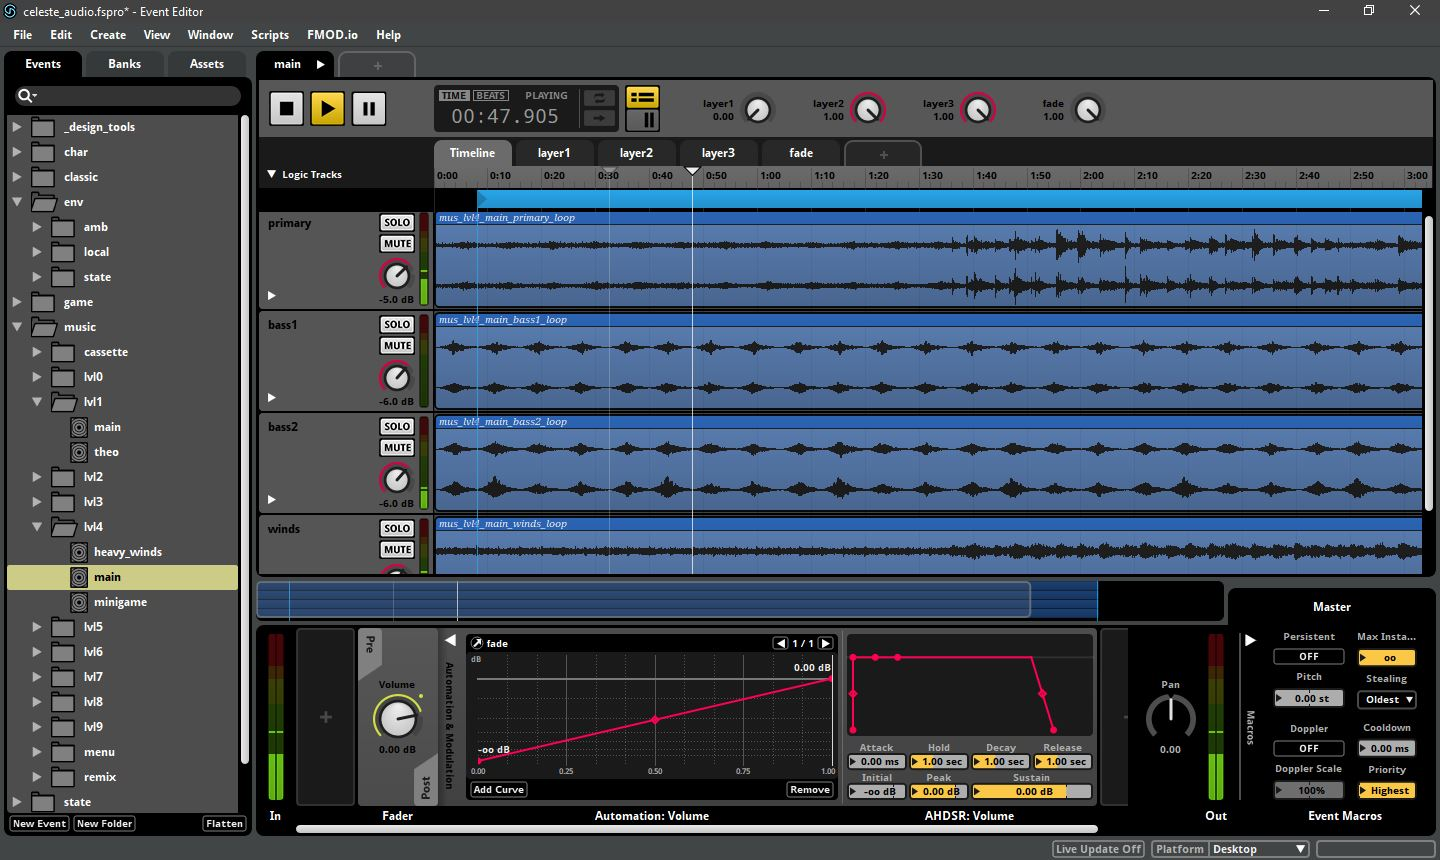
\includegraphics[width=0.6\linewidth]{./Figuras/Aspectos/FMODStudio.jpg}
	\caption{Interfaz de usuario de FMOD Studio.}
	\label{fig:FMODUI}
\end{figure}

A diferencia del sistema de audio de Unity, que tiene funcionalidades limitadas, FMOD Studio permite gestionar con gran precisión las pistas de audio en eventos, incluso utilizando filtros de diversos tipos si fuera necesario. Desde FMOD Studio, se pueden añadir parámetros asociados a zonas de bucle, compases musicales o pistas, que luego pueden ser modificados desde los propios componentes de Unity o por programación de scripts en función de las necesidades del videojuego que se esté desarrollando.

\subsection{TeXstudio}

TeXstudio es un editor de LaTeX de código abierto lanzado en 2009 que ofrece un soporte moderno para la escritura. Cuenta con funcionalidades como la corrección ortográfica interactiva, el plegado de código y el resaltado de sintaxis. La decisión de utilizar un editor de LaTeX en lugar de editores de texto convencionales, como Word, se basa en la magnitud del documento. La citación y referencia automáticas de figuras o tablas que ofrece LaTeX proporciona estabilidad y sostenibilidad al documento. Además, cuando se combina con la distribución Miktex, permite la instalación automática de paquetes y la actualización a las últimas versiones tanto de los paquetes como del propio TeXstudio.

\subsection{GitHub}

GitHub es un repositorio que utiliza el control de versiones de Git para alojar proyectos. Tiene integración directa con Unity y LaTeX, por lo que ha sido muy útil para permitir el trabajo remoto entre los distintos miembros del grupo de investigación e incluso para trabajar en distintos dispositivos sin necesidad de migrar manualmente el proyecto.